\documentclass{article} % For LaTeX2e
\usepackage{nips12submit_e,times}
%\documentstyle[nips12submit_09,times,art10]{article} % For LaTeX 2.09
%\newtheorem{observation}{Observation}
%\newtheorem{claim}{Claim}
%\newtheorem{conjecture}{Conjecture}
%\newtheorem{problem}{Problem}
%\newtheorem{algo}{Algorithm}
%\newtheorem{definition}{Definition}
%\newtheorem{lemma}{Lemma}
%\newtheorem{theorem}{Theorem}
%\newtheorem{proof}{Proof}
%\newtheorem{defi}{Definition}

\newcommand\independent{\protect\mathpalette{\protect\independenT}{\perp}}
\def\independenT#1#2{\mathrel{\setbox0\hbox{$#1#2$}%
\copy0\kern-\wd0\mkern4mu\box0}} 

\newcommand{\atiter}[2]{{#1}^{(#2)}}
\newcommand{\itert}[1]{{#1}^{(t)}}
\newcommand{\itertO}[1]{{#1}^{(t+1)}}
\newcommand{\iiter}[1]{{#1}^{(i)}}
% \newcommand{\raiseTheta}[1]{\theta^{#1}}
\newcommand{\raisePsi}[1]{\psi^{#1}}
\newcommand{\order}[1]{\mathcal{O}(#1)}

\newcommand{\hide}[1]{}
\newcommand{\comment}[1]{\textcolor{red}{{\small #1 }}}
\newcommand{\semihide}[1]{{\tiny #1}}
\newcommand{\reminder}[1]{{\textsf{\textcolor{red}{[#1]}}}}
\newcommand{\makeclean}{
    \renewcommand{\reminder}[1]{}
}

%\newcommand{\QED}{ \hfill {\bf QED}}
\newcommand{\tight}{ \setlength{\itemsep}{-1.0\itemsep} }
    % makes lists tighter

\usepackage[mathscr]{eucal} %% For \mathscr
\usepackage{amsbsy} %% For \boldsymbol
\newcommand{\tensor}[1]{\boldsymbol{\mathscr{#1}}}   %% Tensor macro from Tammy
% \newcommand{\tensor}[1]{{\boldmath\mathcal{#1}}}
\newcommand{\B}[1]{\mathbf{#1}}   %% Tensor macro from Tammy
%\newcommand{\tensor}[1]{\underline{\mathbf{#1}}}  
%\newcommand{\tensor}[1]{\mathbf{\EuScript{#1}}}  
%\newcommand{\tensor}[1]{\mathbf{\mathcal{#1}}}  
\newcommand{\loss}{\mathcal{L}}  

\newcommand{\krp}[2]{ \left( \mathbf{#1}\odot\mathbf{#2} \right)}

\def\blambda{\mbox{\boldmath ${\lambda}$}}

\newcommand{\method}{\textsc{METHOD}\xspace}
\newcommand{\methodplain}{METHOD\xspace}
\newcommand{\graphlab}{GraphLab\xspace}
\newcommand{\psgd}{PSGD\xspace}
\newcommand{\dsgd}{DSGD+\xspace}
\newcommand{\lda}{LDA\xspace}
\newcommand{\dl}{DL\xspace}
\newcommand{\mmsb}{MMSB\xspace}
\newcommand{\twitter}{TGraph\xspace}
\newcommand{\nytimes}{NyTimes\xspace}
\newcommand{\snytimes}[1]{NyTimes{#1}\xspace}
\newcommand{\scaleblenytimes}{Scalable NyTimes\xspace}
\newcommand{\pubmed}{PubMed\xspace}
\newcommand{\imagenet}{ImageNet\xspace}

\newcommand{\sgd}{SGD\xspace}

%\newcommand{\explosion}{\textsc{Idex}\xspace}
\newcommand{\explosion}{intermediate data explosion\xspace}
\newcommand{\Explosion}{Intermediate Data Explosion\xspace}
\newcommand{\gtscaleup}{100\xspace}

\newcommand{\samplecube}{\textsc{ParCube}\xspace}
\newcommand{\parafac}{\textsc{Parafac}\xspace}
\newcommand{\sparafac}{\textsc{Parafac SLF}\xspace}
\newcommand{\merge}{\textsc{Merge}\xspace}
\newcommand{\sample}{\textsc{BiasedSample}\xspace}
\newcommand{\enron}{\textsc{Enron}\xspace}
\newcommand{\facebook}{\textsc{Facebook}\xspace}
\newcommand{\lbnl}{\textsc{Lbnl}\xspace}
\newcommand{\nell}{\textsc{Nell}\xspace}
\newcommand{\argmin}{\text{argmin}\xspace}
\newcommand{\brain}{\textsc{BrainQ}\xspace}


\newcommand{\hadi}{{\cal HADI}\xspace}
\newcommand{\mapreduce}{\textsc{MapReduce}\xspace}
\newcommand{\map}{\textsc{Map}\xspace}
\newcommand{\reduce}{\textsc{Reduce}\xspace}
\newcommand{\combine}{\textsc{Combine}\xspace}
\newcommand{\hadoop}{\textsc{Hadoop}\xspace}
\newcommand{\anf}{\emph{Centralized Method}}
% \newcommand{\MFB}{{MF-bitstring}}
\newcommand{\MFB}{{FM-bitstring}}
\newcommand{\mfb}{{b}}
\newcommand{\MFV}{{FM-vector}}
\newcommand{\mfv}{{\bf v}}
% \newcommand{\mfbhi}{{MF-vector}}
\newcommand{\mfbhi}{{ b(h,i) }}
\newcommand{\Nhi}{N(h,i)}   % number of neighbors of $i$, within h hops or less
\newcommand{\NNhi}{ {\cal N}(h,i)} % SET of neighbors ....
\newcommand{\NNhhi}{ {\cal N}(h+1,i)} % SET of neighbors ....
\newcommand{\NNhj}{ {\cal N}(h,j)} % SET of neighbors ....
\newcommand{\hatmfbhi}{ $\hat{b}(h,i)$} %partial bitmask

\newcommand{\PassA}{{\tt Stage1}\xspace}
\newcommand{\PassAMap}{{\tt Stage1-Map}\xspace}
\newcommand{\PassARed}{{\tt Stage1-Reduce}\xspace}
\newcommand{\PassB}{{\tt Stage2}\xspace}
\newcommand{\PassBMap}{{\tt Stage2-Map}\xspace}
\newcommand{\PassBRed}{{\tt Stage2-Reduce}\xspace}
\newcommand{\PassC}{{\tt Stage3}\xspace}
\newcommand{\PassCMap}{{\tt Stage3-Map}\xspace}
\newcommand{\PassCRed}{{\tt Stage3-Reduce}\xspace}

\newcommand{\diameter}{{\tt diameter}}
\newcommand{\npairs}{{\tt npairs}}
\newcommand{\gcc}{{\tt gcc}}
\newcommand{\entropy}{{\tt entropy}}
% \newcommand{\nedges}{{\tt nedges}}
\newcommand{\sv}{{\mbox{$\lambda_1$}}}
\newcommand{\avgd}{{\tt avgd}}

% math symbol definitions
\newcommand{\mat}[1]{{\bf{#1}}}
\newcommand{\nnodes}{N}     % number of nodes
\newcommand{\nedges}{E}     % number of edges
\newcommand{\deff}{{d_{eff}}}   % effective diameter
\newcommand{\Er}{{E_{r}}}   % number of retained edges
\newcommand{\Nr}{{N_{r}}}   % number of retained nodes
\newcommand{\Nc}{{N_c}}   % number of nodes at critical point
\newcommand{\Ec}{{E_c}}   % number of nodes at critical point
\newcommand{\Ngcc}{{N_{gcc}}} % number of nodes in gcc, at critical poing
\newcommand{\NPairc}{{N_{NPAIRS}}} % number of reachable pairs, at critical poing
\newcommand{\dc}{{d_{c}}} % diameter at critical point
\newcommand{\Lambdac}{{\lambda_{c}}} % First eigenvalue at critical point
% \newcommand{\RED}{ {\em RED } } % random edge deletion
% \newcommand{\FED}{ {\em FED } } % friendly edge deletion
% \newcommand{\HED}{ {\em HED } } % hostile edge deletion
\newcommand{\join}{\texttt{combine2}}
\newcommand{\aggrnp}{\texttt{combineAll}}
\newcommand{\aggr}{\texttt{combineAll$_i$}}
\newcommand{\aggrsid}{\texttt{combineAll$_{E.sid}$}}
\newcommand{\assign}{\texttt{assign}}



\newcommand{\ben}{\begin{enumerate*}}
\newcommand{\een}{\end{enumerate*}}
\newcommand{\bit}{\begin{itemize*}}
\newcommand{\eit}{\end{itemize*}}

% shorthands
\newcommand{\citationsds}{{CITATIONS}}
\newcommand{\epinionsds}{{EPINIONS}}
\newcommand{\patentsds}{{PATENTS}}
\newcommand{\net}[1]{{\textsc{#1}}}

\newcommand{\QED}{\hfill $\Box$ \hfill}





% graph segment
% Notation macros
\newcommand{\G}{\ensuremath{{\mathcal G}}}  % graph stream
\newcommand{\ES}[1]{\ensuremath{m^{(\!#1\!)}}}
%\newcommand{\ES}[1]{\ensuremath{|E|^{(\!#1\!)}}}
\newcommand{\coll}{\ensuremath{\ell}}  % number of source/row groups
\newcommand{\rowk}{\ensuremath{k}}  % number of dest/col groups
\newcommand{\rgrp}[1]{\ensuremath{I^{(\!#1\!)}}}  % node set for src/row group
\newcommand{\cgrp}[1]{\ensuremath{J^{(\!#1\!)}}} % node set for dst/col group
\newcommand{\rgsz}[1]{\ensuremath{l^{(\!#1\!)}}}  % size of node set for src/row group
\newcommand{\cgsz}[1]{\ensuremath{n^{(\!#1\!)}}  }% size of node set for dst/col group
\newcommand{\subG}[1]{\ensuremath{{\mathcal G}^{(\!#1\!)}}}  % submatrices
\newcommand{\den}[1]{\ensuremath{\rho^{(\!#1\!)}}}   % density/probability
\newcommand{\KL}[2]{\ensuremath{{\mathcal D}(#1\|#2)}}   % KL-divergence
\newcommand{\ceil}[1]{\ensuremath{\lceil\!#1\!\rceil}}   % density/probability

\newcommand{\myrot}[1]{\rotatebox[origin=ll]{75}{{#1}}} 


\usepackage{amsmath}%,amsthm}
\usepackage{amsfonts}
\usepackage{amssymb}
\usepackage{subfigure, fink, grffile, placeins}
\usepackage[pdftex]{graphicx} 
\usepackage{epstopdf}
\usepackage{hyperref}
% \usepackage[colorlinks,pagebackref]{hyperref}
% \usepackage[pagebackref]{hyperref}
\usepackage[usenames,dvipsnames]{xcolor}
%\usepackage{algorithmicx,algpseudocode,algorithm}
\usepackage{algorithm2e}
\usepackage{url}
% \usepackage[boxed,noend]{algorithm2e}
%\usepackage{mdwlist}    % from christos / mary: makes lists tighter
%\usepackage{epsfig}
%\usepackage{times}
%\usepackage{setspace}
%\usepackage[pdftex]{graphicx}
%\usepackage[pdftex]{geometry}

%\usepackage{algorithm}
%%\usepackage{algorithmic}
%\usepackage{algpseudocode}
%\usepackage{program}


\newtheorem{observation}{Observation}
\newtheorem{conjecture}{Conjecture}
\newtheorem{problem}{Problem}
\newtheorem{algo}{Algorithm}
\newtheorem{definition}{Definition}
\newtheorem{lemma}{Lemma}
\newtheorem{theorem}{Theorem}
%\newtheorem{question}{Question}
\newtheorem{example}{Example}
%\newtheorem{answer}{Answer}
%\newtheorem{proof}{Proof}

\newcommand{\abhi}[1]{\textcolor{orange}{abhi-comment: #1}}
\newcommand{\alex}[1]{\textcolor{red}{\\ alex-comment: #1}}
\newcommand{\qirong}[1][1]{\textcolor{fuschia}{\\ qirong-comment: #1}}
\newcommand{\eric}[1][1]{\textcolor{blue}{\\ eric-comment: #1}}

\title{Slow-learner Isn't My Problem: Exploiting Structure in
high-D, high-V Latent Space Stochastic Learning}
% \title{Community Discovery through Optimization}


\author{Abhimanu Kumar~~~~~~Alex Beutel~~~~~~Qirong Ho~~~~~~Eric P. Xing 
\\ School of Computer Science, Carnegie Mellon University 
\\ Pittsburgh PA 15213,USA,\\
\{\href{mailto:abhimank@cs.cmu.edu}{abhimank},\href{mailto:abeutel@cs.cmu.edu}{abeutel},
\href{mailto:qho@cs.cmu.edu}{qho},
\href{mailto:epxing@cs.cmu.edu}{epxing}\}@cs.cmu.edu}
% \authorrunning{Kumar et al.}
% The \author macro works with any number of authors. There are two commands
% used to separate the names and addresses of multiple authors: \And and \AND.
%
% Using \And between authors leaves it to \LaTeX{} to determine where to break
% the lines. Using \AND forces a linebreak at that point. So, if \LaTeX{}
% puts 3 of 4 authors names on the first line, and the last on the second
% line, try using \AND instead of \And before the third author name.

\newcommand{\fix}{\marginpar{FIX}}
\newcommand{\new}{\marginpar{NEW}}

\nipsfinalcopy % Uncomment for camera-ready version

\begin{document}


\maketitle

\begin{abstract}
	We pesent here a scheme for exploiting distributable structure present in
	latent space model for high-dimensional (high-D) and high-volume (high-V)
	learning. Models like latent dirichlet allocation and mixed membership
	stochastic blockmodels have structures that can be exploted for big learning.
	We present a distributed learning strategy for such models. The scheme is
	distributed in data as well as parameter space and avoids waiting for slow
	learners to obtain full distributive leverage.
	The learning scheme, flexible to slow worker-processors, has
	provably correct strategy for convergence even with fewer synchronizations.
	It provides a tunable synchronization startegy that can be set based on the
	learning needs of the end user. We provide theoretical bounds on the parameter
	variance among workers with different synchronization strategies. Empirical
	results presented for latent space models such as latent dirichlet allocation 
	and mixed membership model show that it scales very well with large data
	as well as parameter space. The comaparative evaluation with other parallel
	and distributed learning startegies shows better preformance of the model.
	
\end{abstract}

\section{Introduction}
In todays information age there is trillions of bytes of data being generated
every moment. By one estimate we generate 5 exabytes of data on the internet every two
days~\footnote{\url{http://techcrunch.com/2010/08/04/schmidt-data/}} 
and most of
it is user generated content. Given this massive amount of data generated
every moment large scale machine learning is not just of academic
interest anymore but of practical significance too. Large scale learning or big
learning has been an active area of research in recent times. But most of this
research has been focused around big data and the aspect of distibuting the
learnig model has take back seat. While dealing with big data is definitely a must in this massive
content generation age the learning task might turn out to be non-trivial when
big data meets complex models. Learning models with high dimension or number of
parameters becomes non-trivial even with slight increase in data. 
Hence there is a need for learning scheme which can perform distributed data as
well as parameter learning. This problem is highly prevalent in latent space 
model such as latent dirichlet allocation (LDA~\cite{Blei:2003:LDA}), mixed
membership stochastic blockmodels (MMSB~\cite{Airoldi:2008:MMS}) as they inflate
their parameter space by introducing large number of latent variables.
Henceforth these models would be our object of focus in this paper. We develop a
stochastic learning scheme for latent space model, specifically for LDA and
MMSB, which is distributed in data as well as parameter space. We modify the
originial objective to suit our optimization scheme.\comment{need to write this
in a better way}. The structure obtained can be further exploited to minimize
the hazardous effects of slow-processors in the distributed system.  

\comment{expand some more giving an over view of our learning scheme}
\section{Related Work}
\comment{PSGD (only data parallel); Aggarawal and Duci's Distributed Delayed
(Again Data partition only; and it's hard to code); Any Other?}
\comment{How do we discuss the original Haas's paper though we do considerable
more in terms of theory and multi-iteration}

\section{Slow-Learner Agnostic Distributed Learning Framework}

Our approach is to exploit independent cliques of structure present in large
scale machine learning models. Probabilistic graphical models introduce massive
amount of latent variables to induce the modelers belief regarding the
generative process of the data. Though this enables these models with a unique
ability to provide an interpretation and a generative story, it also makes the
model harder to learn since the parameter as well as variable space increases
massively. These models when run on large data have their learning problem
becomes twice difficult. 

While it may appear that latent space models' biggest boon
of incorporating hidden variables is their biggest bane for large scale
learning, it turns out that is not the case. On close examination it appears
that these latent variables have another adavantage: they have a structure. They
are generally found in cliques of correlated variable sets. This independence
structure can be exploited effectively for a distributed learning framework.
Moreover in models such as LDA and MMSB with a modified objective \comment{need to
put it in a better way} one can achieve ditributivity in data as well as
parameters. We explain this using a basic LDA model. In simple terms, the aim of
an LDA model given a \emph{ document by vocabulary} matrix ($Y$) is to split it
into two matrices: a \emph{ documents by topics} ($\pi$) and a \emph{ topics by
vocabulary}  matrix ($\beta$). Equation~\ref{eqn:LDA} presents this in an
optimization framework with simplex and non-negativity constraints. The is an
$\ell_p$ norm which is typecally $\ell_2$.
\begin{eqnarray}
\argmin_{\pi,\beta}L=||Y-\pi\beta||_p^p = \sum_{i,j}(Y_{i,j}-\sum_k
\pi_{i,k}\beta_{j,k})_p^p \label{eqn:LDA}\\
s.t.\sum_k\pi_{i,k}=1,\sum_k\beta_{j,k}=1, \pi_{i,k}\geq 0,
\beta_{j,k}\geq 0~~\forall~ i,j 
\nonumber
\end{eqnarray} 

For MMSB a similar objective can be formulated. Given a \emph{ user by user}
interaction strength \comment{is it the right term} matrix $Y$ it aims to find
two matrices $\pi$ and $B$, which are \emph{user by topic} and \emph{topic by
topic} matrix respectively, such that $\pi^TB\pi$ reconstructs the original
matrix interaction matrix $Y$. Equation~\ref{eqn:MMSB} presents this in an
optimization framework with the usual non-negativity and simplex constraints. 

\begin{eqnarray}
\argmin_{\pi,B}L=||Y-\pi^TB\pi||_p^p = \sum_{i,j}(Y_{i,j}-\sum_{g,h}
\pi_{i,g}B_{g,h}\pi_{j,h})_p^p \label{eqn:MMSB}\\
s.t.\sum_k\pi_{i,k}=1,\pi_{i,k}\geq 0, B_{i,k}\geq 0~~\forall~ i,j \nonumber
\end{eqnarray}

\comment{Do we present the symmetric matrix factorization objective too; since
it's is nice scheduling scheme as well as $\ell_p$ and $\ell_2$ combined loss}

For the LDA objective, figure~\ref{fig:para-div} shows the way parameters are
divided in the distributive scheme. We perform parameter updates of different
blocks parallely. For SGD we perform updates to our parameters $\mathbf{\pi,
\beta}$, which we will collectively refer to as $\bold{\Theta}$ matrix whereas
$\theta$ are the individual components of the matrix. This definition of 
$\bold{\Theta}$ and $\theta$ will come in handy for parameter updates based on
the gradient at individual data points.
E.g. the update for the LDA objective $L$ are (\comment{note: projections are
involved here}):
\begin{align}
\theta^{(t+1)}&= \theta^{(t)} - \eta_t \nabla
\loss_{Y_{i,j}}(\theta^{(t)})
\label{equ:sgd-update-lda}
\end{align}

\begin{figure}
\begin{center}
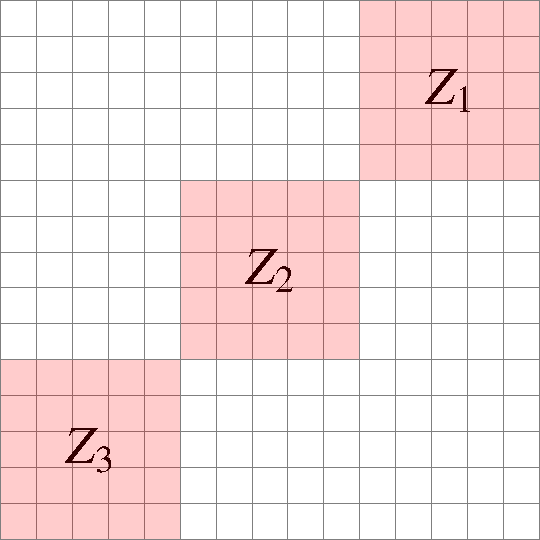
\includegraphics[width=0.2\textwidth]{fig/2dblocks.pdf}
\vspace{-4mm}
\caption{Dividing the \emph{document by vocabulary} matrix fo LDA into blocks
such that no two of them share any row or a column.}
\end{center}
\label{fig:para-div}
\end{figure}

For these update rules, we list below the differentials for each component
$\sigma$ of $\theta$ where norm use is $\ell_2$, and $(\nabla
L_{Y_{i,j}}(\theta))_\sigma = \frac{\partial L_{Y_{i,j}}}{\partial \sigma}$:
\begin{align}
	(\nabla L_{Y_{i,j}}(\theta))_\sigma &= 
	\left\{
	\begin{array}{ll}
		-2(Y_{i,j}-\sum_r \pi_{i,r}\beta_{j,r}
		)\beta_{j,\ell}  & \mbox{if } \sigma = \pi_{i,\ell} \\
		0 & \mbox{if } \sigma = \pi_{i',\ell},\ i\neq i'\\
	\end{array}
	\label{eqn:diff-lda}
\right.
\end{align}
similarly for $\sigma=\beta_{j,l}$. 
From this we observe that SGD update for $\pi_{i,l}$ at a particular entry
$Y_{i,j}$ depends only on previous $\pi_{i,r},
\beta_{j,r}$ where $r\in {1,\ldots,R}$ and $R$ is the number of topics we chose.
The updates for each component are similar for the MMSB case. \comment{modify
here for MMSB}

\begin{algorithm}
Input : $Y,\beta, \pi$,~sub-epoch~size~$d$\\
$\pi\leftarrow \pi_0$, $\beta\leftarrow \beta_0$\\
Block $Y,\pi,\beta$ into corresponding $w$ blocks\\
\While{not converged}{
Pick step size $\eta$\\
% 	\For{$s=0,...,d^2-1$}{
%		\\\*sub-epoch\*\\\\
		Pick $w$ blocks($Z^{(s)}_{1},...,Z^{(s)}_{w}$) to form stratum $Z^{(s)}$\\
		\For{$b=0,\ldots,w-1$ \textbf{in parallel}}{
			Run SGD on the training points $Z^{(s)}_{b}$\\
			/\/** Do unitl every block is ready to synchronize **/\\\
			/\/** So potentially each block $Z^{(s)}_{b}$ runs through each data-point
			$n_{Z^{(s)}_{b}}$ times **/\\\
		}
% 	}
}
\caption{Algorithm for LDA updates. The $w$ blocks correspond to $w$ worker
processors}
\label{algo:lda}
\end{algorithm} 

Given this understanding of our optimization objective and SGD update rules, we
would like to segment our data in such a way that certain blocks $Z_b$ can be
run in parallel, where we define $Z_b \subseteq Y$.
Figure \ref{fig:para-div} sjows the way we segment
our simple matrix $Y$ to enable parallelization. 
In order to run SGD on our blocks in parallel, we divide them such that no two
blocks share common rows or columns.  To be more precise, we say that a point
$y \in Z_b$ is the coordinates in the data, such as $y = (y_i,y_jy) \in
Y$.  Two blocks $Z_b$ and $Z_{b'}$ are non-overlapping if
for all $x \in Z_b$ and
$y' \in Z_{b'}$, $y_i \neq y'_i$ and $y_j \neq y'_j$.
In order to cover all regions of
$Y$, we need multiple strata. We require $w$ strata
In our algorithm, we run the strata sequentially, but for each stratum we run
SGD on the blocks in parallel. Different blocks in a starta can make different number
of passes trhough the data. This is where the algorithm is robust against slow
processors as the worker keep running instead of waiting until every body is
ready to synchronize. We consider running SGD on one stratum to be a subepoch
in our algorithm, and running it on all strata an epoch.  (Note, the order in 
which you run the strata does not matter, as long as they are each run once per 
epoch.)  Algorithm \ref{algo:lda} explain the steps more formally.
We next offer a proof that this multi-iteration per block distributed
parameter learning converges appropriately.





\comment{Our Learning framework presented here. We present it in a way that
emphasizes on latent space models\\} 
\comment{Salient points: \\
1) different processors can make different number of iterations 
over the data without synchronization. \\
2) The workers donot wait for slower workers and instead keep
working and synchronize when everybody is ready. We should add that one
can choose to not synchronize often based on how much they want variance among
different processors and how slow is their slowest processor.\\
3) We present theoretical guaranties for convergence; **for simple as well
as projected loss**\\
4) We provide bounds on variance among different workers at epoch and
sub-epoch levels.\\
5) We demonstrate theoretically that keep doing work in place of waiting gets
faster convergence. **TODO** \\
% (Use potential energy tehnique) 
6) We show that our results are for generic loss fucntion and works
even with projections/constraints($\ell1$, Non-negativity, Simplex etc.)\\
7) **Our assumptions: The structure; Martingale Diference Error $\varepsilon$}


\section{Theoretical Analysis}
\comment{\\ 1) Convergence (with projection)\\
2) Epoch variance bound\\
3) Sub-epoch variance bound\\
4) Show that waiting is not a good idea and workers should keep working till
every one is ready\\}

Here we analyse the method presented in algorithm~\ref{algo:lda} theoretically.
We will prove that the multi-iteration per block strategy converges. We
provide a bound on the variance accross two blocks with in a sub-epoch
running parallely. We show theoretically how the variance varies 
after each synchronization between two consecutive epochs. In the end we show
why working instead of wating for the slowest processor is a better strategy. 

\subsection{Converegnce proof}
Suppose we have $\itert{V}=\itert{V}(\itertO{\theta},\itert{\theta})$ is a
fucntion that keeps track of the state of $\itert{\theta}$ and $\itertO{\theta}$ and depends
upon the data-point $\itert{Y_{i,j}}$ picked in the SGD update.
From equation~\ref{equ:sgd-update-lda} we have
\begin{eqnarray}
\itertO{\theta} &=& \itert{\theta} - \eta_t\delta
\itert{L}(\itert{V},\itert{\theta}) \nonumber\\ %\Longrightarrow \itertO{\theta} 
&=& \itert{\theta} - \eta_t\nabla
\mathcal{L}(\itert{\theta}) + \eta_t\left[ \nabla\mathcal{L}(\itert{\theta}) -
\delta \itert{L}(\itert{V},\itert{\theta})\right] \nonumber\\
 &=& \itert{\theta} - \eta_t\nabla
\mathcal{L}(\itert{\theta}) + \eta_t\varepsilon_t
\end{eqnarray} 
 
Here $ \nabla\mathcal{L}(\itert{\theta})$ is the exact gradient at iteration
$t$. And we call error at iteration $t$, $\left[
\nabla\mathcal{L}(\itert{\theta}) - \delta
\itert{L}(\itert{V},\itert{\theta})\right]$, as $\varepsilon_t$. We make the
assumption that the error $\varepsilon_t=\left[
\nabla\mathcal{L}(\itert{\theta}) - \delta
\itert{L}(\itert{V},\itert{\theta})\right]$ in each step is a martingale
difference sequence. i.e we assume that 
\begin{eqnarray}
E\left[\nabla\mathcal{L}(\itert{\theta}) - \delta
\itert{L}(\itert{V},\itert{\theta})|\delta
\iiter{L}(\iiter{V},\iiter{\theta}),\iiter{\theta},i<t,\itert{\theta}\right] &=&
0 \nonumber \\
E\left[\varepsilon_t|\varepsilon_i,i<t\right] &=& 0
\label{eqn:martingaleAssumption}
\end{eqnarray} 
\comment{Move the following justification of martingale sequence some where
more relevant} We have to note here that assuming error terms are a martingale
difference sequence is a weaker assumption than assuming error terms are independent of
each other. Making the martingale difference assumption means that $\delta
\itert{L}(\itert{V},\itert{\theta})$ conditioned on $\theta^{(0)}$ and $\delta
\iiter{L}(\iiter{V},\iiter{\theta}),\iiter{\theta}$ given $\itert{\theta}$ is
independent of everything else. This is achieved since in the blocking strategy
explained earlier has no overlap between two parameters that are updated
parallely. 

We have $w$ worker processors (algorithm~\ref{algo:lda}) and assume that every
worker $i$ touches each data point $n_i$ times in its block before syncing.
Hence 
\begin{align}
\theta^{(t+(\sum_1^w n_i)m)} = \itert{\theta} + \sum_{i=t}^{t+m(\sum_1^w n_i)}
-\eta_i\mathcal{\nabla L}(\iiter{\theta}) +  \sum_{i=t}^{t+m(\sum_1^w n_i)}
\eta_i\varepsilon_i \nonumber\\
\Longrightarrow \theta^{(t+mN_w)} = \itert{\theta} + \sum_{i=t}^{t+mN_w}
-\eta_i\mathcal{\nabla L}(\iiter{\theta}) + \sum_{i=t}^{t+mN_w}
\eta_i\varepsilon_i \nonumber\\ 
\text{assuming~$\sum_1^w n_i=N_w$} \nonumber \\
\Longrightarrow \theta^{(t+mN_w)} = \itert{\theta} + \sum_{i=t}^{t+mN_w}
-\eta_i\mathcal{\nabla L}(\iiter{\theta}) + M_{mN_w}
\end{align}

where $M_{mN_w}=\sum_{i=t}^{t+mN_w} \eta_i\varepsilon_i$ is a martingale
sequence since it is a sum of martingale difference sequence. Besides $mN_w$
captures the $m$ whole sub-epochs of work done as a whole by all the workers combined.
From Doobs martingale inequality (\cite{Friedman:1975}, ch. 1, Thm 3.8)
\begin{equation}
P\left(\sup_{t+mN_w\geq r \geq t}|M_r|\geq c\right) \leq \frac{E\left[\left(
\sum_{i=t}^{t+mN_w}\eta_i\varepsilon_i\right)^2\right]}{c^2}
\label{eqn:doobs}
\end{equation}

where $M_r=\sum_{i=t}^r\eta_i\varepsilon_i$. Lets look at the RHS of
equation~\ref{eqn:doobs} above:
\begin{align}
E\left[\left(\sum_{i=t}^{t+mN_w}\eta_i\varepsilon_i\right)^2\right] &=
E\left[\sum_{i=1}^{mN_w}\left(\eta_i\varepsilon_i\right)^2\right]
\nonumber\\\text{(equation~\ref{eqn:martingaleAssumption}
$\Longrightarrow~E[\varepsilon_i \varepsilon_j]=0$ if $i\neq j$)}\nonumber\\
=\sum_{i=1}^{mN_w}\eta_i^2E[\varepsilon_i^2] &\leq
\sum_{i=1}^{mN_w}\eta_i^2D \to 0 \nonumber\\
\text{where $E[\varepsilon_i^2]<D~\forall i$ and assuming $\sum\eta_i^2 <\infty$
} \nonumber\\ 
\lim_{t\to\infty}\Longrightarrow P\left(\sup_{i\geq t}|M_i|\geq c\right) =
0~~as~~t\to\infty
\label{eqn:asymptotoError}
\end{align}

From equation~\ref{eqn:asymptotoError} we have
\begin{equation}
\theta^{(t+mN_w)} = \itert{\theta} + \sum_{i=t}^{t+mN_w}
-\eta_i\mathcal{\nabla L}(\iiter{\theta})
\end{equation}
asymptotically. Hence the algorithm converges to the same set of limit poits as
the ecxact gradient descent asymptotically.



% \subsection{Variance Pointwise}
% \comment{Not done fully; we will remove it anyways due to space crunch, besides
% the other epoch and sub-epoch variance bounds are based off of this} 
% Here
% $\atiter{\theta}{t}$ is the value of parameter theta at iteration $t$ and $\atiter{V}{t}(\atiter{\theta}{t+!},\atiter{\theta}{t})$ is a state function
% that is dependent upon the past $\atiter{\theta}{t}$, future
% $\atiter{\theta}{t+1}$ and the data points $\atiter{x}{t}$ picked at iteration.
% $\eta_t$ is the step size at iteration $t$ and $\atiter{L}{t}$ is the
% loss at point $\atiter{x}{t}$ in iter $t$.
% \begin{eqnarray}
% \atiter{\theta}{t+1} = \atiter{\theta}{t} +
% \delta\atiter{\theta}{t}(\atiter{V}{t},\atiter{\theta}{t}) 
% \end{eqnarray}
% ~where~
% \begin{eqnarray}
% \delta\atiter{\theta}{t}(\atiter{V}{t}, \atiter{\theta}{t}) =
% -\atiter{\eta}{t}\delta\atiter{L}{t}(\atiter{V}{t},\atiter{\theta}{t})
% \end{eqnarray}
% Also we have 
% \begin{eqnarray}
% & & p(\itertO{\theta}|\itert{\theta})\partial\itertO{\theta} =
% p(\itert{V}(\itertO{\theta},\itert{\theta}))\partial\itert{V} \nonumber\\
% \Longrightarrow & &  p(\itertO{\theta})\partial\itertO{\theta} =
% \int_{\itert{\theta}} p(\itertO{\theta}|\itert{\theta}) p(\itert{\theta})
% \partial\itert{\theta} \partial\itertO{\theta}
% % \Longrightarrow & & \\
% % \Longrightarrow & & \\
% % \Longrightarrow & & \\
% \end{eqnarray}
% Now lets evaluate $E^{\itertO{\theta}}[\bar{Y}(\itertO{\theta})]$ where
% $\bar{Y}(\theta)$ is some function of $\theta$.
% 
% \begin{eqnarray}
% E^{\itertO{\theta}}[\bar{Y}(\itertO{\theta})] &=& \int_{\itertO{\theta}}
% \bar{Y}(\itertO{\theta}) p(\itertO{\theta})\partial\itertO{\theta} \nonumber\\
% & = & \int_{\itert{V}}\int_{\itert{\theta}}\bar{Y}(\itertO{\theta})
% p(\itert{V}(\itertO{\theta},\itert{\theta}))\partial\itert{V}p(\itert{\theta})
% \partial\itert{\theta} \nonumber \\
% &=&\int_{\itert{\theta}} \left( \int_{\itert{V}}\bar{Y}(\itertO{\theta})
% p(\itert{V}(\itertO{\theta},\itert{\theta}))\partial\itert{V} \right) p(\itert{\theta})
% \partial\itert{\theta} \nonumber \\
% & = & E^{\itert{\theta}\left[E^{\itert{V}}\left[\bar{Y}(\itertO{\theta})
% \right]\right]}
% \end{eqnarray} 

\subsection{Variance in a Sub-epoch}
Here
$\atiter{\theta}{t}$ is the value of parameter theta at iteration $t$ and 
$\atiter{V}{t}(\atiter{\theta}{t+!},\atiter{\theta}{t})$ is a state function
that is dependent upon the past $\atiter{\theta}{t}$, future
$\atiter{\theta}{t+1}$ and the data points $\atiter{x}{t}$ picked at iteration.
$\eta_t$ is the step size at iteration $t$ and $\atiter{L}{t}$ is the
loss at point $\atiter{x}{t}$ in iter $t$. We assume for simplicity that the
parameter being updated in block-$i$ is univariate. This analysis can be
easily extended to a multivariate parameter updation case in each block of a
sub-epoch.

\begin{align}
\atiter{\theta}{t+1} = \atiter{\theta}{t} -
\delta\atiter{\theta}{t}(\atiter{V}{t},\atiter{\theta}{t}) 
\label{eqn:iterDelta1} \\
%\end{eqnarray}
\text{where 
$\,\delta\atiter{\theta}{t}(\atiter{V}{t}, \atiter{\theta}{t}) =
\atiter{\eta}{t}\delta\atiter{L}{t}(\atiter{V}{t},\atiter{\theta}{t})\Rightarrow
\raiseTheta{(t+1)} = \raiseTheta{t} - \eta_{t} \delta L^{t} \! (v^{t},
\raiseTheta{t})$} \nonumber\\
\text{Summing equation~\ref{eqn:iterDelta1} over $n_i$, the number of points in
block $i$ of a sub-epoch} \nonumber\\
\raiseTheta{t+n_{i}} = \raiseTheta{t} - \sum_{i=1}^{n_{i}} \! \eta_{t+i} \delta
L^{t+i}(v^{t+i}, \theta^{t+i})
\end{align}

 

\begin{align}
p(\raiseTheta{(t+1)}|\raiseTheta{t}) d\raiseTheta{(t+1)} &= 
p(u(\raiseTheta{(t+ni)}, \raiseTheta{t})) du~~p(\raiseTheta{(t+ni)})
d\raiseTheta{(t+ni)} \nonumber\\ 
&= \int_{\raiseTheta{t}} \!
p(\raiseTheta{(t+ni)}|\raiseTheta{t}) p(\raiseTheta{t}) d \raiseTheta{t} 
d \raiseTheta{(t+ni)}
= \int_{\raiseTheta{t}} \! p(V(\raiseTheta{(t+ni)}, \raiseTheta{t})) dV 
d\raiseTheta{t}
\end{align}

\begin{align}
\mathbb{E}^{\raiseTheta{(t+n_i)}}[u(\raiseTheta{(t+n_i)})] &= 
\int_{\raiseTheta{(t+n_i)}} \! u(\raiseTheta{(t+n_i)}) p(\raiseTheta{(t+n_i)}) d 
\raiseTheta{(t+n_i)} \nonumber\\
&= \int_{\raiseTheta{t+i}} 
\! u(\raiseTheta{(t+n_i)}) P(\raiseTheta{(t+n_i)}) d\raiseTheta{(t+n_i)}\nonumber\\
&= \int_{V} \! \int_{\raiseTheta{t}} \! u(\raiseTheta{(t+n_i)}) P(V(\raiseTheta{(t+n_i)}, \theta)) 
dV P(\raiseTheta{t}) d\raiseTheta{t}\nonumber\\
&= \mathbb{E}^{\raiseTheta{t}}[\mathbb{E}^{V}[u(\raiseTheta{(t+n_i)})]]
\label{eqn:expectNewTheta}
\end{align}

\begin{align}
&\mathbb{E}^{V}[u(\theta^{(t+ni)})] = \mathbb{E}^{V}[u(\theta^{t} +
(-\underbrace{\sum_{i=1}^{n_{i}} \! \eta_{t+i} \delta L^{t+i} (v^{t+i},
\theta^{t+i})}_{\nabla}))] \nonumber\\
& = \mathbb{E}^{V}[u(\theta^{t}) - \frac{du(\theta^{t})}{d\theta^{t}}\nabla +
\frac{1}{2}\frac{du^2(\theta^{t})}{d(\theta^{t})^2}\nabla^2 + \order{\eta_t^3}]
\nonumber\\
& = u(\theta^{t}) -
\eta_t\frac{du(\theta^{t})}{d\theta^{t}}\mathbb{E}^{V}[\sum_{i=1}^{n_{i}} \!
\delta L^{t+i} (v^{t+i}, \theta^{t+i})] %\nonumber \\
%& 
+ \eta_t^2\frac{1}{2}\frac{du^2(\theta^{t})}{d(\theta^{t})^2}
\mathbb{E}^{V}[(\sum_{i=1}^{n_{i}} \! \delta L^{t+i} (v^{t+i}, \theta^{t+i}))^2]
\nonumber \\ &\,+ \order{\eta_t^3} %\nonumber\\
%& 
~~~~~~~~~~\text{\Bigg(since $\eta_t=\eta_{t+i}$ within a block\Bigg) }
\nonumber\\
&= u(\theta^{t}) -
\eta_t\frac{du(\theta^{t})}{d\theta^{t}} \sum_{i=1}^{n_{i}}
\frac{d\mathbb{E}^{V}[L^{t+i} (v^{t+i},
\theta^{t+i})]}{d\theta^{t+i}} %\nonumber\\
%& 
+ \eta_t^2\frac{1}{2}\frac{du^2(\theta^{t})}{d(\theta^{t})^2}
\mathbb{E}^{V}[(\sum_{i=1}^{n_{i}} \! \frac{dL^{t+i} (v^{t+i},
\theta^{t+i})}{d\theta^{t+i}})^2] \nonumber\\ 
&\,+ \order{\eta_t^3}\nonumber\\
& = u(\theta^{t}) - \eta_t\frac{du(\theta^{t})}{d\theta^{t}}
(n_i\frac{d\mathbb{E}^{v^t}[L^{t} (v^{t}, \theta^{t})]}{d\theta^{t}})
%\nonumber\\
%&
~~~~~~~~~~\text{\Bigg(by expectation property} \nonumber\\
&\text{ 
$\mathbb{E}^{V}[L^{t+i} (v^{t+i},\theta^{t+i})] = \mathbb{E}^{v^{t+i}}[L^{t+i}
(v^{t+i},\theta^{t+i})] = \mathbb{E}^{v^t}[L^{t}
(v^{t},\theta^{t})]$,} \nonumber\\ &\text{\& assuming the condition that we make
small and equal gradient step in each iteration } \nonumber\\ &\text{$(t+i)$ in
the same direction i.e.
$\frac{d\mathbb{E}^{v^{t+i}}[L^{t+i}
(v^{t+i},\theta^{t+i})]}{d\theta^{t+i}} = \frac{d\mathbb{E}^{v^{t+j}}[L^{t+j}
(v^{t+j},\theta^{t+j})]}{d\theta^{t+j}}$\Bigg)}\nonumber\\
& + \eta_t^2\frac{1}{2}\frac{du^2(\theta^{t})}{d(\theta^{t})^2}
\bigg[\mathbb{E}^{V}[\sum_{i=1}^{n_{i}} (\frac{dL^{t+i} (v^{t+i},
\theta^{t+i})}{d\theta^{t+i}})^2] %\nonumber \\ 
%&
+ \mathbb{E}^{V}[\sum_{i\neq
j}\! \frac{dL^{t+i} (v^{t+i}, \theta^{t+i})}{d\theta^{t+i}}\frac{dL^{t+j} (v^{t+j},
\theta^{t+i})}{d\theta^{t+j}}]\bigg]\nonumber \\ 
&\, 
+\order{\eta_t^3} \nonumber \\
& = u(\theta^{t}) - \eta_t\frac{du(\theta^{t})}{d\theta^{t}}
(n_i\frac{d\mathbb{E}^{v^t}[L^{t} (v^{t}, \theta^{t})]}{d\theta^{t}})
%\nonumber\\
%& 
+ \eta_t^2\frac{1}{2}\frac{du^2(\theta^{t})}{d(\theta^{t})^2}
\bigg[\sum_{i=1}^{n_{i}}\mathbb{E}^{v^t}[(\frac{dL^{t+i} (v^{t+i},
\theta^{t+i})} {d\theta^{t+i}})^2] \nonumber \\
&+ n_i(n_i-1)(\frac{d\mathbb{E}^{v^t}[L^{t} (v^{t},
\theta^{t})]}{d\theta^{t}})^2\bigg] +
\order{\eta_t^3} 
\label{eqn:expectV}
\end{align}

Last statement in equation~\ref{eqn:expectV} holds because two different data
points picked at iteration $(t+i)$ and $(t+j)$ are independent of each other, by
expectation property
\begin{equation}
\mathbb{E}^{V}[\frac{dL^{t+i} (v^{t+i},
\theta^{t+i})}{d\theta^{t+i}}\frac{dL^{t+j} (v^{t+j}, \theta^{t+i})}
{d\theta^{t+j}}] = \mathbb{E}^{v^{t+i}}[\frac{dL^{t+i} (v^{t+i},
\theta^{t+i})]}{d\theta^{t+i}}]\mathbb{E}^{v^{t+j}}[\frac{dL^{t+j} (v^{t+j},
\theta^{t+i})} {d\theta^{t+j}}]
\label{eqn:covIndependent} 
\end{equation}

From equation~\ref{eqn:expectV} and~\ref{eqn:expectNewTheta}
\begin{align}
\mathbb{E}^{\raiseTheta{(t+n_i)}}[u(\raiseTheta{(t+n_i)})] &=
\mathbb{E}^{\raiseTheta{(t)}}\bigg[ u(\theta^{t}) -
\eta_t\frac{du(\theta^{t})}{d\theta^{t}} (n_i\frac{d\mathbb{E}^{v^t}[L^{t} (v^{t}, \theta^{t})]}{d\theta^{t}}) \nonumber\\
& + \eta_t^2\frac{1}{2}\frac{du^2(\theta^{t})}{d(\theta^{t})^2}
[\sum_{i=1}^{n_{i}}\mathbb{E}^{v^t}[(\frac{dL^{t+i} (v^{t+i}, \theta^{t+i})}
{d\theta^{t+i}})^2] \nonumber \\
&+ n_i(n_i-1)(\frac{d\mathbb{E}^{v^t}[L^{t} (v^{t},
\theta^{t})]}{d\theta^{t}})^2] \bigg] +
\order{\eta_t^3}
\end{align}


From equation above the variance of $\raiseTheta{t+n_i}$ is
\begin{align}
&Var(\raiseTheta{t+n_i}) =
\mathbb{E}^{\raiseTheta{(t+n_i)}}[(\raiseTheta{(t+n_i)})^2] - \left(\mathbb{E}^{\raiseTheta{(t+n_i)}}[\raiseTheta{(t+n_i)}]\right)^2
\nonumber\\ 
&= \mathbb{E}^{\theta^t}[(\theta^t)^2] - \eta_t n_i
\mathbb{E}^{\theta^t}[2\theta^t(C_0(\theta^t-\theta_*) +
\order{|\theta^t-\theta_*|^2})] \nonumber\\
&+
\eta_t^2\frac{1}{2}\mathbb{E}^{\theta^t}[2\{n_i^2(C_1+C_2\epsilon_t+\order{\epsilon_t^2})
+ n_i(n_i-1)(C_0(\theta^t-\theta_*)+\order{|\theta^t-\theta_*|^2})^2\}]
\nonumber\\
&- \left(\mathbb{E}^{\theta^t}[(\theta^t)^2] - \eta_t n_i
\mathbb{E}^{\theta^t}[2\theta^t(C_0(\theta^t-\theta_*) +
\order{|\theta^t-\theta_*|^2})]\right)^2 \nonumber\\
& = \mathbb{E}^{\theta^t}[(\theta^t)^2] - 2C_0\eta_t n_i
\mathbb{E}^{\theta^t}[(\theta^t)^2] +
2C_0\eta_tn_i\theta_*\mathbb{E}^{\theta^t}[\theta^t] -
\order{\eta_t\epsilon_t^2} \nonumber\\ 
&+ \eta_t^2n_i^2C_1 +
n_i^2C_2\order{\eta_t^2\epsilon_t} + \order{\eta_t^2\epsilon_t^2} \nonumber \\
&-\left(\mathbb{E}^{\theta^t}[\theta^t]\right)^2 +
2n_i\eta_t\mathbb{E}^{\theta^t}[\theta^t](\mathbb{E}^{\theta^t}[C_0\theta^t]
-C_0\theta_* +\order{|\theta_t-\theta_*|^2}) - \order{\eta_t^2\epsilon_t^2}
+\order{\eta_t^3} \nonumber \\
&=Var(\theta^t)- 2\eta_tn_iC_0(Var(\theta^t)) + \eta_t^2n_i^2C_1 +
\order{\eta_t^2\epsilon_t} + \order{\eta_t\epsilon_t^2} + \order{\eta_t^3}
\label{eqn:varBoundBlock}
\end{align}



\comment{Make clear that we are simplifying here and making the assumption that
$\theta$ is uni-variate}
\subsection{Variance between two consecutive sub-epochs}
From our algorithm defined 

\subsection{Why waiting is bad}

\section{Experiments}
\comment{This is the part that we need to decide very early}

\subsection{Scalability experiments in data as well as parameter}
\comment{Experiments to show how it scales with more processors (Do we have enough
processors?) a) Scaling with parameters (number of topics), and b) Scaling with
Data (Documents)} 


\subsection{Speed comparison and less sycnhing experiments}
\comment{\\ Comparison with PSGD on the speed and accuracy of convergence (Do
we compare on the original objective or the new objective)\\}

\subsection{Qualitative results on latent space models} 
\comment{\\We do both for MMSB and LDA both\\}
\comment{\\Qirong and Alex think that we should include symmetric matrix
factorization as well as it shows the scheduling strategy when thinsg are not cleanly
seperated.}
\section{Results Analaysis and Discussion}

\section{Conclusion}



\bibliography{biblio}
\bibliographystyle{plain}
\end{document}
